% QA correction 11-26-2026: finding g7-M2; historical captions retained.
% Appendix 9b: Concordance identity, score-then-calibrate baselines, rank optimization diagnostics, LoRA weight training, and human-rating summary.
% Provenance: Exp 06, Exp 07, Exp 08 (including results/ce_gradient_check.json), Exp 09, and Exp 10.
% One sentence per line (Trigger Rule 13); strictly anonymized.

\section{Concordance Identity, Calibration Baselines, and Human-Rating Summary}
\label{app:concordance}

\subsection{Concordance Identity and Psychometric Connections}
Let $x = (x_1, \dots, x_N)$ denote predicted expected ratings and $y = (y_1, \dots, y_N)$ denote human target ratings, with sample means $\bar{x}, \bar{y}$ and population standard deviations $s_x, s_y$.
Expanding the mean squared error yields Lin's concordance identity~\citep{lin1989concordance}:
\begin{equation}
\label{eq:lin-concordance}
\frac{1}{N} \sum_{i=1}^{N} (x_i - y_i)^2 = (\bar{x} - \bar{y})^2 + (s_x - s_y)^2 + 2 s_x s_y (1 - r_{x,y}).
\end{equation}
Pearson correlation $r_{x,y}$ constrains only the third term.
Any positively scaled affine shift $x'_i = a x_i + b$ with $a > 0$ leaves $r_{x,y}$ invariant while inflating the bias term $(\bar{x} - \bar{y})^2$ and scale mismatch $(s_x - s_y)^2$.
Consequently, scalar standardization of Pearson predictions recovers neither signed offset nor variance amplitude unless calibrated against raw human targets.

Equation~\eqref{eq:lin-concordance} parallels classical reliability splits in psychometrics.
Specifically, McGraw and Wong~\citep{mcgraw1996forming} separate relative consistency $\mathrm{ICC}(\mathrm{C},1)$, which ignores additive rater shifts, from absolute agreement $\mathrm{ICC}(\mathrm{A},1)$, which penalizes both mean bias and scale discrepancy.
Likewise, many-facet ordinal likelihood models with explicit rater parameters~\citep{linacre1989many} are already proper-loss probability models estimated by likelihood.
Our critique therefore targets selecting or training uncalibrated scalar judges solely via rank or linear correlation, rather than likelihood-based psychometrics at large.

\subsection{Score-Then-Calibrate Baselines and Regularization Diagnostics}
A natural remediation for scalar Pearson training is two-stage calibration: fit weights $W$ by regularized Pearson correlation to extract a one-dimensional score $s(x) = m_W(x)$, standardize $z(x) = (s(x) - \bar{s}) / \mathrm{sd}(s)$ on training tasks, and fit a 12-parameter six-way softmax head $q_{\mathrm{head}}(r \mid x) = \mathrm{softmax}(a_r + b_r z(x))$ via regularized cross-entropy (CE).
Because $b = 0$ recovers the marginal histogram baseline, one might expect this head never to underperform a constant predictor at small $n$.
In synthetic studies reusing a shared $(1/n)\|W\|^2$ ridge in Stage 2 without separate head regularization, however, Stage~1 overfits small samples ($n \le 32$), producing standardized scores $z(x)$ that drive Stage~2 predictions toward extreme categories ($0.0861$--$0.1626$ ranked probability score (RPS) excess in Scenario~A and $0.0914$--$0.2483$ in Scenario~B).
Once regularized properly or given larger $n$, the head closes most of the scale gap ($0.0088$ vs.\ CE $0.0011$ in Scenario~A and $0.0080$ vs.\ CE $0.0042$ in Scenario~B at $n=1{,}024$), yet still cannot recover conditional spread variations orthogonal to $s(x)$.
A dedicated follow-up (Experiment~11) confirms that four-fold cross-fitting of Stage-1 scores paired with validation-selected Stage-2 slope regularization $c_b \in \{0.01, \dots, 10^8\}$ cuts the naive $n \le 32$ calibration spike over constant from $+0.1040$--$+0.1470$ down to $+0.0145$--$+0.0387$ (vanishing by $n=32$: $-0.0004$ to $+0.0006$ across Scenarios~A--D).
Directly training all 78 softmax weights via mean squared error (MSE) also fixes Pearson's scale drift ($0.0076$--$0.0118$ RPS excess at $n=2{,}048$), yet still underperforms validation-tuned CE ($0.0007$--$0.0036$) because MSE constrains only the conditional mean.
Moreover, whereas properly regularized 12-parameter Stage-2 CE heads slightly edge out unconstrained 78-weight CE when concentration $\kappa$ is constant ($0.0015$--$0.0022$ vs.\ $0.0027$--$0.0029$ RPS excess in Scenarios~C and~D at $n=2{,}048$), they remain bounded well above CE whenever disagreement $\kappa(x)$ varies ($0.0078$--$0.0079$ vs.\ $0.0007$ in Scenario~A; $0.0071$--$0.0074$ vs.\ $0.0036$ in Scenario~B).

\paragraph{Correction to restart descriptions (11-26-2026).}
The earlier descriptions said ``100 seeds'', ``best-of-9'' and ``9 starts''; the stored experiment 07 records instead contain 30 seeds and five starts per correlation objective (the original start plus four random ones, chosen by the training objective; one CE start), with 540 records in total, and the figure image already stated this.
The figure caption, the paragraph after it and the caption of Table~\ref{tab:restarts-conv} were updated on 11-28-2026 to the stored values.

\begin{figure}[t]
\centering
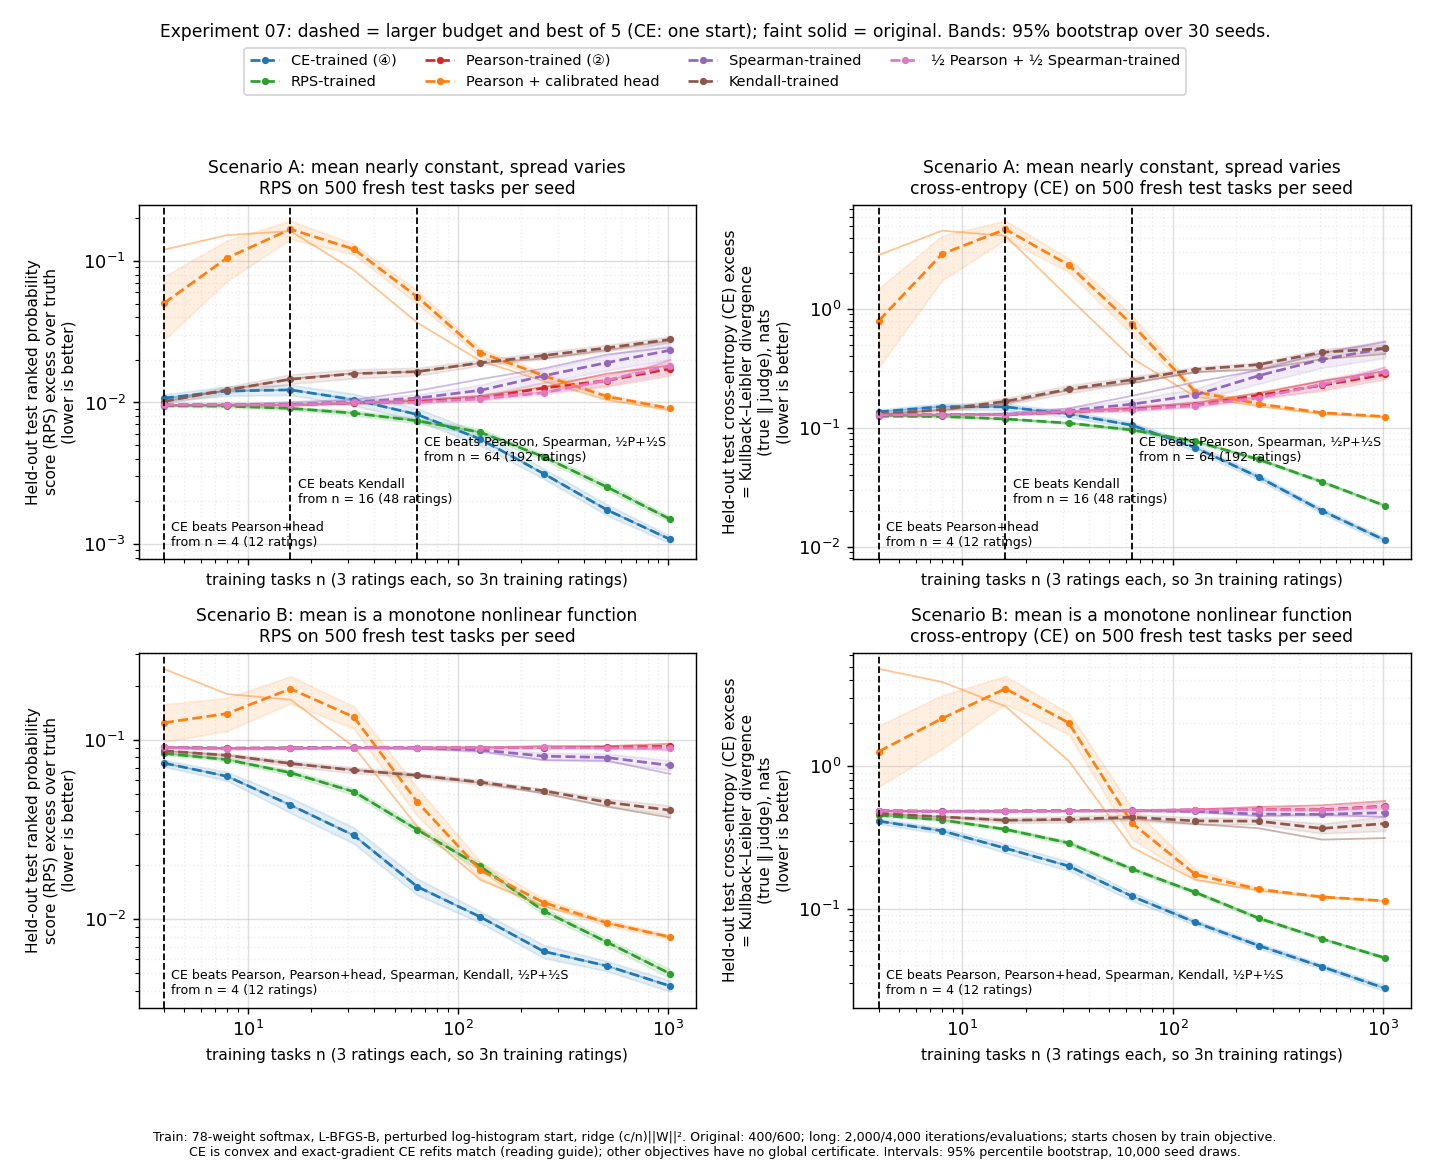
\includegraphics[width=\columnwidth]{figures/fig_restarts_vs_n.png}
\caption{Held-out test RPS excess and CE excess versus training tasks $n$ (each with 3 ratings; 500 test tasks per seed across 30 seeds) comparing single-start fits against best-of-5 multi-start restarts (the original start plus four random ones, chosen by the training objective; L-BFGS-B up to 2,000 iterations) in synthetic Scenarios~A and~B\@.
Convex CE eliminates optimizer sensitivity, whereas Stage-2 calibration spikes at $n \le 32$ before stabilizing near $0.008$--$0.009$ RPS excess at $n=1{,}024$.}
\label{fig:restarts-app}
\end{figure}

Table~\ref{tab:restarts-conv} and Figure~\ref{fig:restarts-app} summarize optimizer reliability across objectives from Experiment~07.
At $n \ge 32$ tasks under the 400-iteration budget, convex CE, smooth RPS, and the 12-parameter calibration head reach full L-BFGS-B convergence on all runs, whereas scale-free Pearson converges on $0\%$ of runs ($91\%$ still exhaust an extended 2,000-iteration cap).
Multi-start restarts (\texttt{best} over 5 starts) improve Pearson by at most $0.001$--$0.003$ RPS excess at $n=1{,}024$, leaving the gap to CE intact.

\begin{table*}[t]
\centering
\caption{Optimizer convergence rates at $n \ge 32$ and Scenario~A/B held-out test RPS excess (\texttt{orig} single-start $\to$ \texttt{best} of 5 starts, 2,000-iteration budget, 30 seeds; 0 optimal, lower is better).}
\label{tab:restarts-conv}
\small
\begin{tabular}{@{}lcc@{}}
\hline
Objective (Search Family) & Convergence ($n \ge 32$) & Held-Out Test RPS Excess (Scenario A / B, $n=1{,}024$) \\
\hline
CE-trained (78-wt softmax) & $100\%$ & $0.0011$ / $0.0042$ \\
RPS-trained (78-wt softmax) & $100\%$ & $0.0015$ / $0.0050$ \\
Pearson + calibrated head (12-p head) & $100\%$ & $0.0088 \to 0.0091$ / $0.0080 \to 0.0079$ \\
Kendall surrogate (78-wt softmax) & $97$--$100\%$ & --- \\
Spearman surrogate (78-wt softmax) & $7$--$52\%$ & --- \\
Pearson-trained (78-wt softmax) & $0\%$ & $0.0183 \to 0.0173$ / $0.0949 \to 0.0918$ \\
\hline
\end{tabular}
\end{table*}

Table~\ref{tab:app-exp08-short} compares validation-selected ridge regularization (Formulations~\textcircled{3} and~\textcircled{1}) against fixed ridge (\textcircled{4} and~\textcircled{2}) across all four synthetic targets of Experiment~08.
Even in Scenario~D with a strictly linear conditional mean, directly training all 78 weights on fixed-ridge Pearson loses to the constant marginal histogram at $n=2{,}048$ ($0.0523$ vs.\ $0.0449$, paired diff $+0.0074$ $[+0.0063, +0.0087]$), whereas validation tuning lowers Pearson to $0.0359$ while proper CE achieves $0.0027$--$0.0028$.
To verify numerical stability, a post-hoc exact-gradient audit (\texttt{ce\_gradient\_check.json}) refitted all $95{,}291$ CE models using analytical log-sum-exp gradients: all $95{,}291$ fits converged, $0/4{,}400$ fixed-ridge grid points moved above $10^{-9}$ (maximum RPS-excess change $1.06 \times 10^{-13}$), and $338/4{,}400$ validation-tuned rows shifted (only one ridge selection change, max RPS-excess shift $0.00023$, and zero changes in condition means or crossovers).

\begin{table*}[t]
\centering
\caption{Experiment~08 held-out test RPS excess over truth across Scenarios~A--D under fixed regularization (\textcircled{4} CE, \textcircled{2} Pearson) and validation-tuned ridge (\textcircled{3} Val-CE, \textcircled{1} Val-Pearson) at $n=4$ and $n=2{,}048$ tasks (lower is better; Pearson minus Constant positive means Pearson loses to the marginal histogram).}
\label{tab:app-exp08-short}
\footnotesize
\setlength{\tabcolsep}{4.5pt}
\begin{tabular}{@{}lcccccc@{}}
\hline
Scenario & Tasks $n$ & Constant & \textcircled{4} CE & \textcircled{3} Val-CE & \textcircled{2} Pearson & \textcircled{1} Val-Pearson \\
\hline
Scenario A (flat mean) & $4$ / $2{,}048$ & $0.0267$ / $0.0096$ & $0.0106$ / $0.0007$ & $0.0140$ / $0.0007$ & $0.0096$ / $0.0253$ & $0.0097$ / $0.0807$ \\
Scenario B (curved mean) & $4$ / $2{,}048$ & $0.0923$ / $0.0670$ & $0.0740$ / $0.0037$ & $0.0829$ / $0.0036$ & $0.0901$ / $0.0951$ & $0.0898$ / $0.0326$ \\
Scenario C (nonlinear mean) & $4$ / $2{,}048$ & $0.0877$ / $0.0640$ & $0.0682$ / $0.0032$ & $0.0776$ / $0.0029$ & $0.0830$ / $0.0893$ & $0.0836$ / $0.0333$ \\
Scenario D (linear mean) & $4$ / $2{,}048$ & $0.0654$ / $0.0449$ & $0.0410$ / $0.0028$ & $0.0481$ / $0.0027$ & $0.0452$ / $0.0523$ & $0.0474$ / $0.0359$ \\
\hline
\multicolumn{7}{@{}p{0.92\textwidth}@{}}{At $n=2{,}048$, \textcircled{2} Pearson minus Constant [95\% CI]: A $+0.0157$ $[+0.0128,+0.0189]$; B $+0.0281$ $[+0.0262,+0.0303]$; C $+0.0252$ $[+0.0237,+0.0268]$; D $+0.0074$ $[+0.0063,+0.0087]$.} \\
\hline
\end{tabular}
\end{table*}

\subsection{LoRA Weight Training and Cross-Study Human-Rating Summary}
Figure~\ref{fig:app-lora} illustrates true neural weight optimization via LoRA adapters on a 4B open-weight judge alongside the concordance MSE decomposition from Equation~\eqref{eq:lin-concordance}.
Directly optimizing LoRA weights for Pearson correlation produces large positive bias ($+1.53$ on the 4B instruction backbone and $+2.11$ on a 7B coder backbone) and high MSE ($4.31$ and $6.43$), driving test RPS to $0.3351$ and $0.4015$.
Proper-loss LoRA fits reach $0.1887$--$0.2007$ RPS on 4B ($0.1821$--$0.1927$ on 7B), and pairing Pearson LoRA features with a 12-parameter CE head eliminates the bias and achieves $0.1412$ RPS ($1.593$ nats) on 4B and $0.1560$ RPS ($1.709$ nats) on 7B\@.

\begin{figure}[t]
\centering
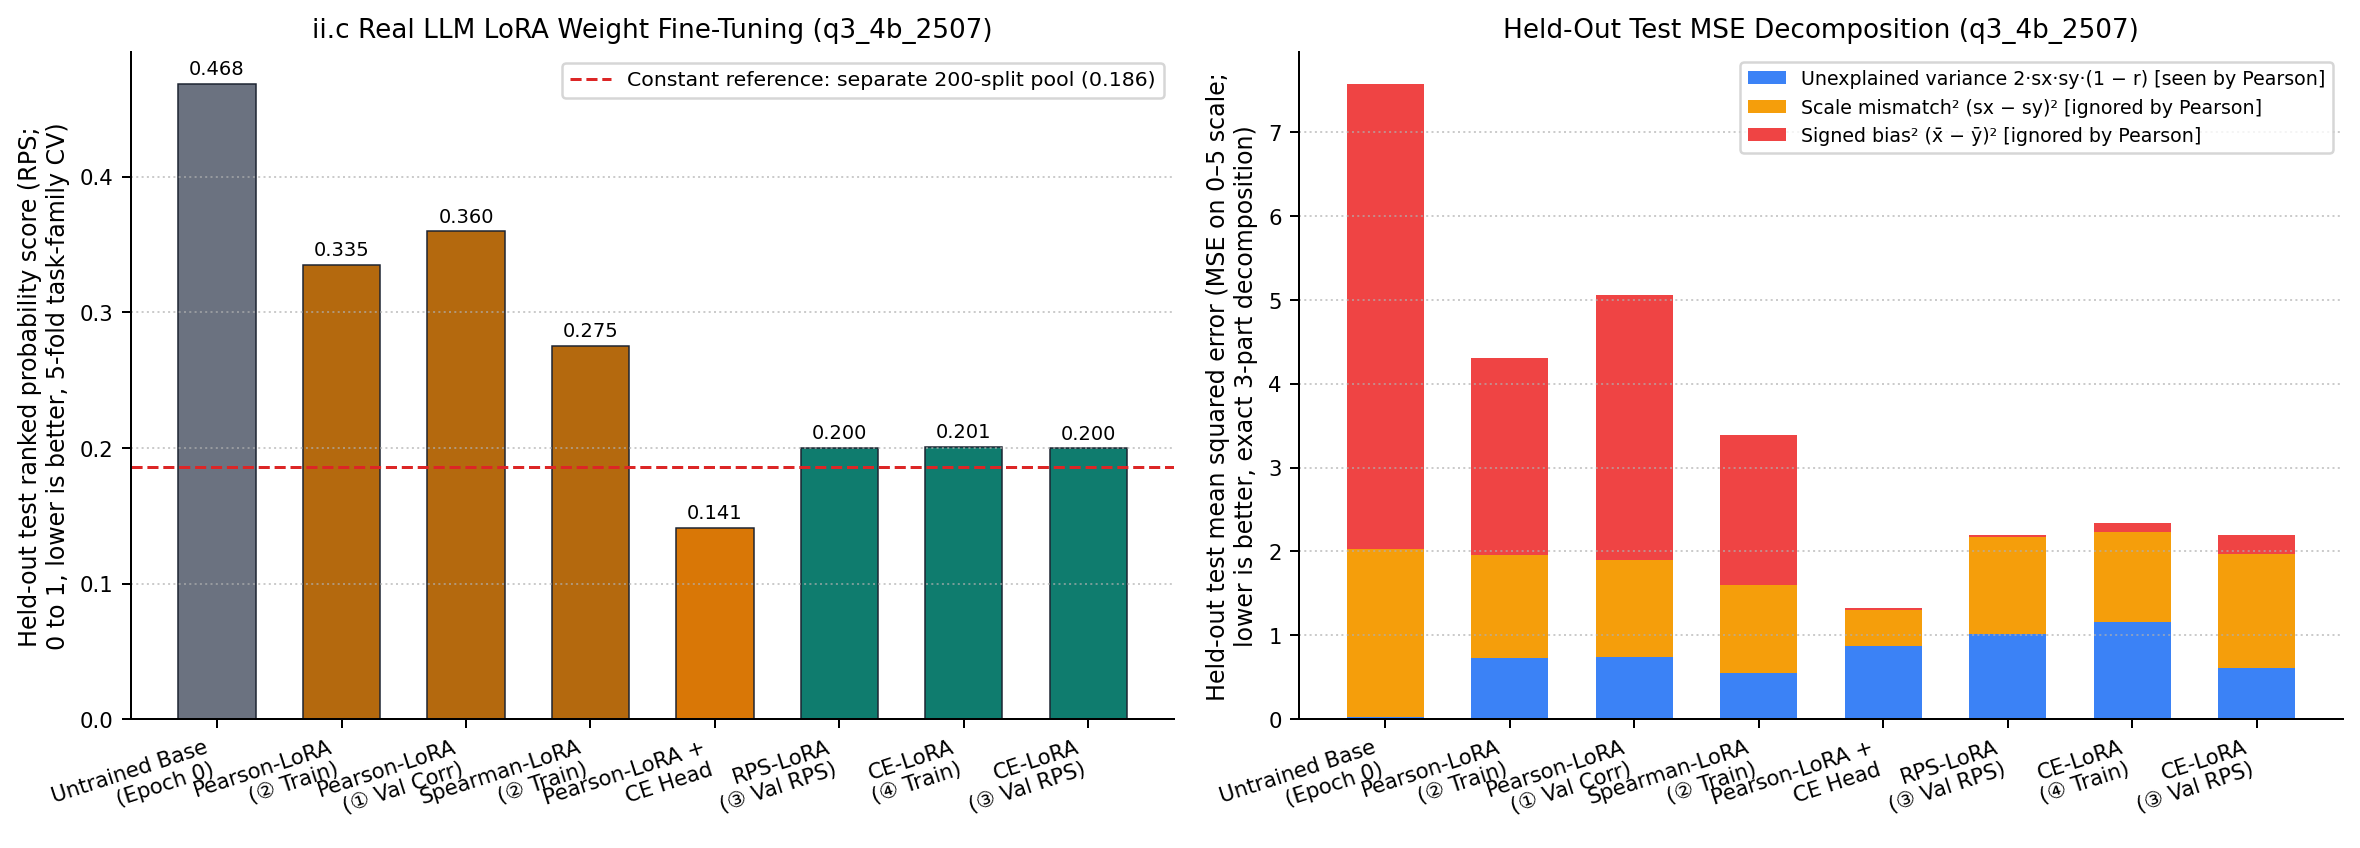
\includegraphics[width=\columnwidth]{figures/fig2_lora_weight_training_and_mse_decomp.png}
\caption{Experiment~09 held-out LoRA weight-training results for a 4B open-weight judge and Lin concordance MSE decomposition across base zero-shot, correlation-trained (Pearson/Spearman), proper-loss (CE/RPS), and Pearson-LoRA + 12-parameter calibrated-head judges on $15/4$ family splits.}
\label{fig:app-lora}
\end{figure}

Table~\ref{tab:human-summary-app} synthesizes all held-out protocols across the retrospective 75-artifact corpus (25 Python tasks, 19 families, 2--3 expert ratings per item; constant baseline $0.1857$--$0.1872$ RPS).
Where single-judge selection operates over coarse pools with raw three-sample histograms under a $10^{-6}$ floor, CE selection absorbs sampling noise ($0.2032$ on 5 historical judges; $0.1869$ on 10 verbal models), whereas proper RPS single-judge selection ($0.1488$ vs.\ $0.1840$, $+0.0352$ $[+0.0098,+0.0639]$) and proper-loss ensembles over native probability outputs consistently outperform both the constant baseline and Pearson selection.
Complete sample-size tables, full rank-surrogate curves, live blind $9/5/5$ prompt-and-harness splits, and data-provenance boundaries appear in the supplementary material.

\begin{table*}[t]
\centering
\caption{Concise cross-study held-out human-rating performance across pooled and single-judge protocols (lower RPS and CE are better; constant baseline $\approx 0.186$--$0.187$ RPS, $\approx 1.89$--$1.93$ nats CE).}
\label{tab:human-summary-app}
\footnotesize
\setlength{\tabcolsep}{2.5pt}
\begin{tabular}{@{}lcc@{}}
\hline
Experiment Pool \& Protocol & Held-Out Test RPS & Key Paired Comparison / Diagnostic \\
\hline
Open-wt Scalar-39 Mix (CE / Pearson) & $0.2819$ / $0.3263$ & Scalar blows up CE ($3.480$ / $5.668$ nats) \\
Open-wt 10-Model Verbal Mix (CE / RPS / P) & $0.1431$ / $0.1433$ / $0.1848$ & RPS/CE mixtures beat Pearson \& constant \\
Open-wt Verbal Single (CE / RPS / P) & $0.1869$ / $0.1488$ / $0.1840$ & RPS single $+0.0352$ $[+0.0098,+0.0639]$ vs.\ P \\
Open-wt 59-Harness Mix (CE / RPS / P) & $0.1325$ / $0.1310$ / $0.1836$ & Mix RPS $+0.0511$ $[+0.0222,+0.0833]$ ($p=.0053$) \\
\hline
LoRA 4B Model (Base / P / CE-tr / RPS-tr) & $0.4683$ / $0.3351$ / $0.2007$ / $0.1887$ & P+12p head reaches $0.1412$ RPS ($1.593$ nats) \\
LoRA 7B Model (Base / P / CE-tr / RPS-tr) & $0.4067$ / $0.4015$ / $0.1927$ / $0.1821$ & P+12p head reaches $0.1560$ RPS ($1.709$ nats) \\
\hline
Frontier Hist-5 (Const / CE-m / RPS-m / P-m) & $0.1872$ / $0.1391$ / $0.1350$ / $0.1436$ & Null mixture difference on 5 scalar judges \\
Frontier Native-15 (CE-m / Val / RPS-m / P-m) & $0.1137$ / $0.1136$ / $0.1166$ / $0.1912$ & Pearson mixture suffers $+1.129$ signed bias \\
Frontier Native-15 Single (CE / RPS / P) & $0.1252$ / $0.1360$ / $0.1426$ & Proper losses edge out single Pearson \\
Frontier Combined-20 (Val-CE / RPS-m / P-m) & $0.1091$ / $0.1093$ / $0.1671$ & Single Pearson $0.1848$ vs.\ CE $0.1091$ mixture \\
\hline
\end{tabular}
\end{table*}
